\documentclass[journal,12pt,twocolumn]{IEEEtran}
%
\usepackage{setspace}
\usepackage{gensymb}
%\doublespacing
\singlespacing

\usepackage{graphicx}
\usepackage[cmex10]{amsmath}
\usepackage{amsmath,amsthm}
\usepackage{mathrsfs}
\usepackage{txfonts}
\usepackage{stfloats}
\usepackage{bm}
\usepackage{cite}
\usepackage{cases}
\usepackage{subfig}

\usepackage{longtable}
\usepackage{multirow}
\usepackage{commath}
\usepackage{enumitem}
\usepackage{mathtools}
\usepackage{steinmetz}
\usepackage{tikz}
\usepackage{circuitikz}
\usepackage{verbatim}
\usepackage{tfrupee}
\usepackage[breaklinks=true]{hyperref}

\usepackage{tkz-euclide}

\usetikzlibrary{calc,math}
\usepackage{listings}
    \usepackage{color}                                            
    \usepackage{array}                                            
    \usepackage{longtable}                                        
    \usepackage{calc}                                             
    \usepackage{multirow}                                         
    \usepackage{hhline}                                           
    \usepackage{ifthen}                                           
    \usepackage{lscape}     
\usepackage{multicol}
\usepackage{chngcntr}

\DeclareMathOperator*{\Res}{Res}

\renewcommand\thesection{\arabic{section}}
\renewcommand\thesubsection{\thesection.\arabic{subsection}}
\renewcommand\thesubsubsection{\thesubsection.\arabic{subsubsection}}

\renewcommand\thesectiondis{\arabic{section}}
\renewcommand\thesubsectiondis{\thesectiondis.\arabic{subsection}}
\renewcommand\thesubsubsectiondis{\thesubsectiondis.\arabic{subsubsection}}

\hyphenation{op-tical net-works semi-conduc-tor}
\def\inputGnumericTable{}                                 

\lstset{
%language=C,
frame=single, 
breaklines=true,
columns=fullflexible
}
\lstset{
%language=TeX,
frame=single, 
breaklines=true
}

\begin{document}


\newtheorem{theorem}{Theorem}[section]
\newtheorem{problem}{Problem}
\newtheorem{proposition}{Proposition}[section]
\newtheorem{lemma}{Lemma}[section]
\newtheorem{corollary}[theorem]{Corollary}
\newtheorem{example}{Example}[section]
\newtheorem{definition}[problem]{Definition}

\newcommand{\BEQA}{\begin{eqnarray}}
\newcommand{\EEQA}{\end{eqnarray}}
\newcommand{\define}{\stackrel{\triangle}{=}}
\bibliographystyle{IEEEtran}
\providecommand{\mbf}{\mathbf}
\providecommand{\pr}[1]{\ensuremath{\Pr\left(#1\right)}}
\providecommand{\qfunc}[1]{\ensuremath{Q\left(#1\right)}}
\providecommand{\sbrak}[1]{\ensuremath{{}\left[#1\right]}}
\providecommand{\lsbrak}[1]{\ensuremath{{}\left[#1\right.}}
\providecommand{\rsbrak}[1]{\ensuremath{{}\left.#1\right]}}
\providecommand{\brak}[1]{\ensuremath{\left(#1\right)}}
\providecommand{\lbrak}[1]{\ensuremath{\left(#1\right.}}
\providecommand{\rbrak}[1]{\ensuremath{\left.#1\right)}}
\providecommand{\cbrak}[1]{\ensuremath{\left\{#1\right\}}}
\providecommand{\lcbrak}[1]{\ensuremath{\left\{#1\right.}}
\providecommand{\rcbrak}[1]{\ensuremath{\left.#1\right\}}}
\theoremstyle{remark}
\newtheorem{rem}{Remark}
\newcommand{\sgn}{\mathop{\mathrm{sgn}}}
\providecommand{\abs}[1]{\(\left\vert#1\right\vert\)}
\providecommand{\res}[1]{\Res\displaylimits_{#1}} 
\providecommand{\norm}[1]{\(\left\lVert#1\right\rVert\)}
%\providecommand{\norm}[1]{\lVert#1\rVert}
\providecommand{\mtx}[1]{\mathbf{#1}}
\providecommand{\mean}[1]{E\(\left[ #1 \right]\)}
\providecommand{\fourier}{\overset{\mathcal{F}}{ \rightleftharpoons}}
%\providecommand{\hilbert}{\overset{\mathcal{H}}{ \rightleftharpoons}}
\providecommand{\system}{\overset{\mathcal{H}}{ \longleftrightarrow}}
	%\newcommand{\solution}[2]{\textbf{Solution:}{#1}}
\newcommand{\solution}{\noindent \textbf{Solution: }}
\newcommand{\cosec}{\,\text{cosec}\,}
\providecommand{\dec}[2]{\ensuremath{\overset{#1}{\underset{#2}{\gtrless}}}}
\newcommand{\myvec}[1]{\ensuremath{\begin{psmallmatrix}#1\end{psmallmatrix}}}
\newcommand{\mydet}[1]{\ensuremath{\begin{vmatrix}#1\end{vmatrix}}}
%\numberwithin{equation}{section}
\numberwithin{equation}{subsection}
%\numberwithin{problem}{section}
%\numberwithin{definition}{section}
\makeatletter
\@addtoreset{figure}{problem}
\makeatother
\let\StandardTheFigure\thefigure
\let\vec\mathbf
%\renewcommand{\thefigure}{\theproblem.\arabic{figure}}
\renewcommand{\thefigure}{\theproblem}
%\setlist[enumerate,1]{before=\renewcommand\theequation{\theenumi.\arabic{equation}}
%\counterwithin{equation}{enumi}
%\renewcommand{\theequation}{\arabic{subsection}.\arabic{equation}}
\def\putbox#1#2#3{\makebox[0in][l]{\makebox[#1][l]{}\raisebox{\baselineskip}[0in][0in]{\raisebox{#2}[0in][0in]{#3}}}}
     \def\rightbox#1{\makebox[0in][r]{#1}}
     \def\centbox#1{\makebox[0in]{#1}}
     \def\topbox#1{\raisebox{-\baselineskip}[0in][0in]{#1}}
     \def\midbox#1{\raisebox{-0.5\baselineskip}[0in][0in]{#1}}
\vspace{3cm}
\title{Assignment 2}
\author{Sairam V C Rebbapragada}
\maketitle
\newpage
%\tableofcontents
\bigskip
\renewcommand{\thefigure}{\theenumi}
\renewcommand{\thetable}{\theenumi}
\begin{abstract}
This document explains the concepts of Matrix transpose, Matrix Equality by solving a problem.
\end{abstract}
Download the python code from 
%
\begin{lstlisting}
https://github.com/Sairam13001/AI5006/blob/master/Assignment_2/assignment_2.py
\end{lstlisting}
%
and latex-tikz codes from 
%
\begin{lstlisting}
https://github.com/Sairam13001/AI5006/blob/master/Assignment_2/assignment_2.tex
\end{lstlisting}
%
\section{Problem}
\begin{align*}
   \vec{A}  = \myvec{ \cos{\alpha} & -\sin{\alpha}\\ \sin{\alpha} & \cos{\alpha}}     
\end{align*}
and $\vec{A}$ + $\vec{A}^\top$ = $\vec{I}$, then find the value of angle $\alpha$.


\section{Explanation}

The Complex number equivalent to the matrix is: 

\begin{align}
\myvec{a & -b\\ b & a } \implies \myvec{a \\ b }
\end{align}
 
\begin{align}
 \vec{A}  = \myvec{ a \\ b }\implies \vec{A}^\top = \myvec{a \\ -b}  
\end{align}



And addition of $\vec{A}$ with $\vec{A}^\top$ results in  :
  
\begin{align}
    \myvec{  a \\ b } + \myvec{ a \\ -b } = \myvec{ 2a \\ 0}
\end{align}

\section{Solution}


So, According to the given question $\vec{A}$ + $\vec{A}^\top$ is : 
\begin{align}
   \myvec{\cos{\alpha} \\ \sin{\alpha}} + \myvec{\cos{\alpha} \\ -\sin{\alpha}} = \myvec{ 2\cos{\alpha} \\ 0} 
\end{align}

Given that  $\vec{A}$ + $\vec{A}^\top$ = $\vec{I}$ :
\begin{align}
  \myvec{2\cos{\alpha} \\ 0} = \myvec{ 1 \\ 0} 
\end{align}

That Implies, 
\begin{align}
 2\cos{\alpha} = 1 \implies \cos{\alpha} = \frac{1}{2}   
\end{align}

As per the cosine values, the angle $\alpha$ is :
\begin{align}
 \alpha =  \frac{\pi}{3} = 1.047
\end{align}
  
The cosine function is plotted along with the point (x, cos(x)) = (1.047, 0.5) as shown in Fig. 0:  
\begin{figure}[h]
    \centering
    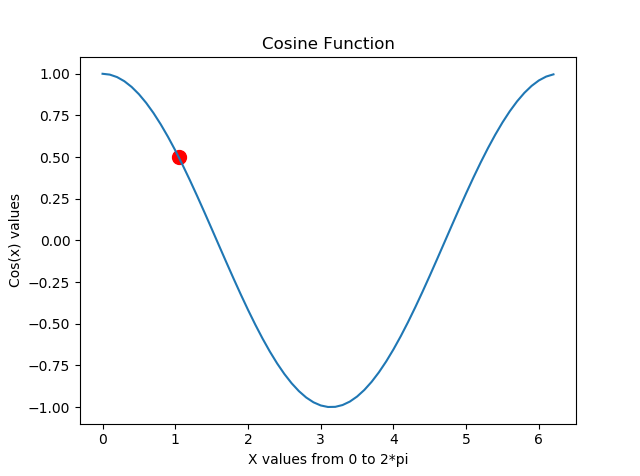
\includegraphics[width=\columnwidth]{assignment_2.png}
    \caption{Cosine Function}
    \label{fig:cosine}
\end{figure}
\end{document}
